% DESIGN
\graphicspath{ {images/} }

In this section I design the design choices made for the application and the
guiding principles behind them. It progresses to show how a graph are visually
displayed and animated in the app without going in the technical details of
implementation. Finally, the intended effect on the user while going through
the various topics explained in the application will be discussed.  I will
also touch on the learning impact of each topic on the user as it forms an
essential aspect of overall design.

\section{Guiding Principles}

\subsection{Simplicity}
\label{design: simplicity}
For the purpose of elucidation of Mathematical concepts, which requires an
undivided attention of the learner, it was decided that the user interface must
have the minimum amount of clutter possible, without sacrificing in terms of the minimum
amount of functionality required. The learner should not get distracted by an
overpopulated user interface. Simplicity and elegance would also lead the user
to stay longer on the application without getting visually exhausted.
Furthermore the users on the web today are extremely goal driven and do not want any
obstruction between them and their goal. \cite{Karvonen2000}

\subsection{Intuitiveness}
The layout of the user interface should be such that it not only has utility,
but should also help communicate the intention of the designer about the usage
of the application. For example a play button, just like it was found on media
devices for decades, invites the user to kick-start an animation even without
going through the instruction which tells him to do so explicitly. The size and
placement of the play button on the page, therefore becomes important. Right
placement of user interactive elements guide the user through the story which
is intended to be told.

\subsection{Meaningfulness}
For a substantial learning impact, the elucidation of the problems must reach at
the heart of the topic. They must have a storyline which is
meaningful and coherent. The learning outcomes of the animation or a
user-interactive task must be well defined before an attempt is made to
implement them.

\section{Wire-frame and Navigation}
The web application is implemented as a \textbf{Single Page Application}. The navigation
from one topic to another occurs according to the user inputs, and when the state
moves from one graph theory to another topic, the data on the screen, that is
the graphics and the text, change on the same page without loading a new HTML page
each time. The user however will notice the url change with navigation from one
topic to another. This will also give the user the ability to use forward and
backward buttons in the browser to navigate through the history of URLs
visited. As a new HTML page is not loaded every time the user navigates from
one topic to another the screen therefore does not turn briefly white and the
transitions are imperceptible by default.

\begin{figure}[H]
    \centering
    \begin{minipage}{.5\textwidth}
        \centering
        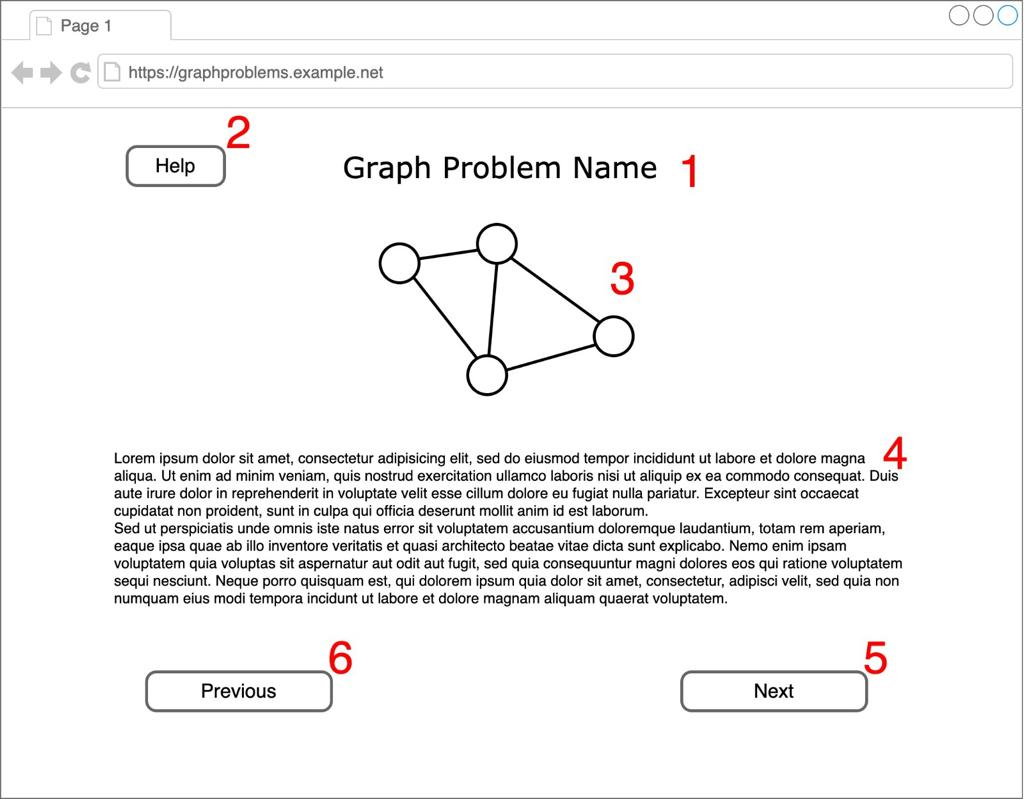
\includegraphics[width=.9\linewidth]{WireframeInitial}
        \caption{An initial wireframe}
        \label{fig:pubsub1}
    \end{minipage}%
    \begin{minipage}{.5\textwidth}
        \centering
        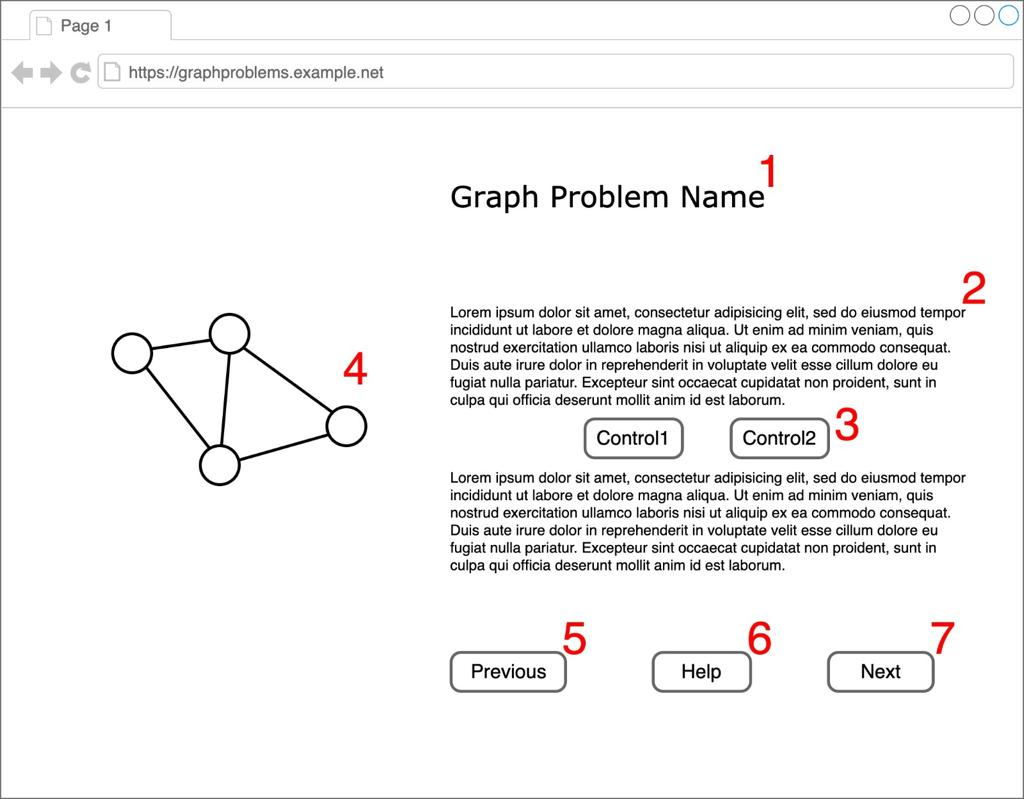
\includegraphics[width=.9\linewidth]{Wireframe}
        \caption{The final wireframe}
        \label{fig:pubsub2}
    \end{minipage}
\end{figure}

There were several iterations made for the layout of the web page, one of the
is shown in \autoref{wireframe: initial}. Finally a more suitable and optically balanced design was selected, see
\autoref{wireframe: final}. On this layout, the page is vertically divided into two
parts, the left part of the page contains an instance of an animation, the
right contains explanation of the topic and advice on how to interpret the
animation along with navigation and control buttons. 

The text in the explanation part of the page is dynamic in nature, if the
animation has facility of user interaction with its elements, the
corresponding text on the right responds with advises on the state of affairs
and what the user should do next.

There is a navigation bar at the bottom of the page, with left and right
arrows, along with the names of the previous and the next topics, to jump from
one topic to another.

\subsection{Home Page, About Page and Header Bar}
\label{design: home}

The home page is the landing page of the application. It gives the user
clickable icons for navigation to the topics. The icons must have the name of
the topic and a miniature graph which best represents the topic. 

The about page has a short description of the purpose of the application with a
short write up introducing the developer and the supervisor of the project. It
also has an acknowledgement section mentioning the people who have been important
in the completion of the project.

Every page has a header bar, which has buttons to navigate to home and about
pages respectively. The bar stays at its place even if the rest of this
page is scrolled down for access to navigation.

\section{Animation Panel} 
As mentioned in the preceding section, the left half of the page is for
graphics, which contains an animation, a user-interaction session or a
combination of both.  The animation contains one or more than one graphs. These
graphs undergo, according to needs of the topic in consideration
transformations of appearance and annotation.

\subsection{Visual representation of graphs} 
The graphs are represented as vertices and edges joining those vertices.
Although the geometrical placement of the vertices is of no consequence in the
subject of graph theory, for the purpose of visualization, vertices are
assigned a two-dimensional position. The edges do not contain attributes such as
length or positions of endpoints of a line segment, they are rather defined as
a relation between a pair of vertices.

\subsubsection{Appearance of Vertices} 

The vertices of graphs in the animations are colour filled circles of the
same size save for certain exceptions. The colour of the vertices have been
allotted by varying mostly the hue and keeping saturation and lightness
relatively same in the \textbf{HSL} (Hue Saturation Lightness) colour space. The
vertices contain a name inside the circle as an integer. The names of vertices
were chosen as integers as it was assumed that such a representation would help
the developer and also the user to keep a track of them as order of integers
may be understood better by users.

When a particular vertex is needed to be shown differently than the rest then
its size and colour are displayed differently. For example, a user-selected
vertex in some of the animations are shown bigger and its colour changed to
golden. The gold colour it was observed makes the vertex in consideration
stand out differently from other colours in the animation.

\subsubsection{Appearance of Edges}
Edges are defined very algebraically as a relationship between a pair
of vertices, but they are simply drawn by connecting the positions of the related vertices with a straight line segment white in colour.

When an edge is supposed to be shown differently than the rest of the edges its
width is increased and colour changed to the same value of golden as a selected vertex.
Again it was found that this colour and thickness, made the edge standout from the
rest of the edges and helped in showing it distinguished without being unpleasantly
distracting.

\section{Explanation Panel}
The animation panel on the left page contains all the graphical
components of the topic elucidation and the right half of the page is occupied by
the Explanation Panel. It contains the title of the problem,
its definition and instruction on how to go ahead with starting the animation
or user-interactive tasks.  It also contains control buttons for starting,
re-starting and pausing animations.  For user-interactive tasks it also shows a button to reset the task.

As the animation or a user-interactive task progresses the explanation panel
generates explanatory and instructive text.

The explanation panel also has navigation panel with buttons to navigate from
one topic to another.

\section{User Stories for Elucidation of Topics}

This section describes, what the user is intended to experience while
interacting with the individual topics in the application with a special
consideration towards learning impact and understandibility.

When the user opens the web application on a browser of her choice, the first
topic she sees is Graph Isomorphism. They may stay there to interact
with the example of the topic or navigate to other topics using navigation
buttons at the bottom to have a bird's eye view of other topics.

Each graph theory problem has its own character and require a different
approach for elucidation. The following sections will explain these approaches
with their intended experience on the user with learning outcomes which may be
achieved.

The survey mentioned in the \autoref{section: selectionCriteria} also gave
quite a few suggestions on different ways to elucidate the short listed topics.
The suggestions were very specific to topics, and included various ideas such as
animations and games and the ability to construct user defined graphs. Some
of the suggestions could be included in the project, some could not be
accomodated as they did not fit the flow of narrative, while others while being
brilliant ideas, act as inspiration for future work due to constraints of time.

\subsection{Graph Isomorphism}
\label{story: isomorphism}
The user is presented with a graph on the left and textual explanation on the
right of the page.  The textual explanation portion of the page also has some
media buttons such as play/pause and reset to control the state of the
animation. The text explanation briefly defines graph isomorphism and advises
the user to press the play button.

\subsubsection{Animation:}
When the user presses the play button, a new graph emerges out of the old one
while the keeping the edges between any two vertices conserved. 
While keeping the connectivity between the vertices intact, the graph
transforms into a completely new shape, almost giving a visual proof that the
two graphs on the screen are isomorphic to each other.

\subsubsection{User Interaction:}
After the two isomorphic graphs have separated from each other, the user is
advised in a text panel to choose a vertex by either hovering over a vertex or
pressing the corresponding number on the keyboard. Doing so will change the
visual appearance of the selected vertex, the edges incident on the selected
vertex and the adjacent vertices to the selected vertex in both graphs.  The
selected vertex will be enlarged to a new radius and change its colour from its
original colour to golden colour making it stand apart from the rest of the
vertices.  The edges incident on the vertex will change their colours to the
same gold colour.  The adjacent vertices to the selected vertex will form a
golden halo around them.  This colour transformation will distinguish a kind of
a subset in the two displayed graphs. At this point, on the text panel
the user is reminded that the selected vertex has the same number of edges
connecting to the same adjacent vertices in both the graphs. The user is also
advised to inspect other vertices of the graphs and note that each
vertex of the graph has the same adjacent vertices in both the isomorphic
counterparts.

\subsubsection{Quiz:}
The user can with a click of a button go to the quiz page which resides within
the topic of Isomorphism. The application asks the user to select a graph (among more than
one graphs) which the user thinks is isomorphic to a given reference graph.  When
they make their choice, they are presented with the right answer along with an animation on
how the correct answer is isomorphic to the reference graph.

\subsubsection{Learning Impact:}
The transformation of a graph into a radically different looking graph but
being essentially the same as far as the connectivity between the vertices go
acts as a visual proof that the graphs are isomorphic, and individually
inspecting each vertex will re-confirm this idea to the user. After having
experienced the concept of graph isomorphism in this way, hopefully the
concept and definition of the term would be clear to the user.


\subsection{Max k Cut}
\label{story: maxkcut}
Max Cut has two animations one after the other. The first animation is about
Max 2 Cut and the second is about Max 3 Cut.  It is assumed that the user will
extrapolate the concept of the general Max k Cut after understanding the first
two cases ($k=2$, $k=3$) and extrapolating it over greater values of k.  The
examples shown in the animations are a nearly bipartite and a tripartite graph
for $k=2$ and $k=3$ respectively.  A nearly bipartite and a tripartite graph is
used to elucidate the topic as it is easier for the user to visualize how the
two graphs can be segregated to sets of vertices such that the maximum number
of edges pass between such sets.

In both the cases of $k=2$ and $k=3$, the weight of all the edges is taken to
be equal to $1$. This decision has been taken as with $w=1$, the answers to
both the max cut problems are more visual than unequal weights.

\subsubsection{Max 2 Cut Animation:} 
\label{story: max2cut}
This animation starts with an Original graph on the left and definition of Max K Cut and
Max 2 Cut on the right of the web page. The right part of the page also
contains media buttons to pause and play the animations. It also has a button
for switching from Max 2 Cut example, to Max 3 Cut example.  The Max 2 Cut
animation starts with a graph, which starts when the user presses the play
button. As the animation progresses a new graph emerges out of the original
one and translates towards the right changing its shape to segregate its
vertices into two sets forming a Maximum 2 Cut. The two sets move vertically up
and down and increase the distance between themselves, revealing the
number of edges passing from one set to another which the user can intuitively
tell is greater than the number of edges between any other two sets
which may have been formed from the vertices of the graph.

The user is advised to put up a pre-defined horizontal line by pressing a
button in the explanation panel. The line is drawn between the two sets of
vertices.  The intersection points between the edges and the max cut line is
shown by blue dots. These user is advised to observe the number of intersection
points which tell the user the number of edges passing from one set to another.

\begin{figure}[h]
\centering
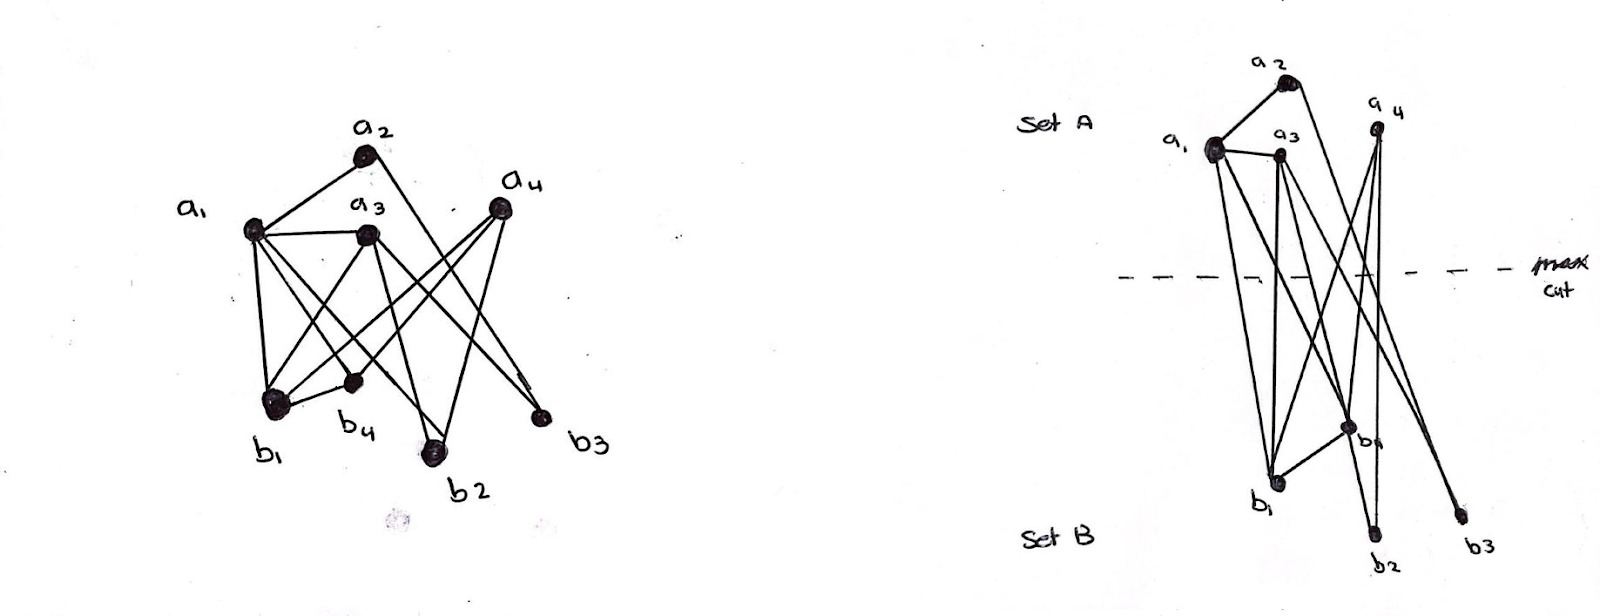
\includegraphics[scale=0.2]{maxcutdes}
\caption{
         Initial design of Max 2 Cut. The initial graph is shown in the left. It
         must go through a transformation such that the two sets of the Max
         Cut are separated form each other as shown in the right. Preferably
         there should be a line between the two sets for visual separation.
        }
\end{figure}

\subsubsection{Max 3 Cut Animation:}
\label{story: max3cut}
Just like the animation for Max 2 Cut, this animation is started by the user by
pressing the play button. The animation on the right starts with a tripartite
graph arranged in a circular form. As the animation progresses the graph gets
Divided into three sets of vertices in which the three sets translate in
directions which are set $120^{\circ}$ apart from each other. The graph
transforms from a circularly arranged one to a triangular form. The user can
draw the Max 3 Cut lines at any point in the progress of the animation.  These
are three lines separating each set from the rest of the graph, with points of
intersection shown in blue showing the number of edges passing from one set to
the rest of the sets.

\subsubsection{Learning Impact:}
Although the examples in the Max 2 Cut and Max 3 Cut can be seen as simple ones
as the first one was nearly a bipartite graph and the second one was a
tripartite graph, I believe they will do a good job at defining the problem. 
Beyond the visualization explaining the problem, they may also have some artistic value in their aesthetic and satisfying appearances, especially in the case of Max 3 Cut, which may inspire an
imaginative student to want to investigate the subject further.


\subsection{Graph colouring}
\label{story: coloring}
\subsubsection{User Interaction:}
User-interactive task was chosen for explaining Graph colouring as the nature
of the problem lends naturally for this implementation. The user is presented with a graph
which has all the vertices in colour white. On the explanation panel to the
right he is given the definition of the problem and advice on how to complete
the task.  

The task is to choose colours from a colour palette of three colours namely red,
green and blue, and colour vertices in the graph such that no two adjacent
vertices have the same colour. Whenever the user colours two or more adjacent
vertices the same colour the text panel warns them to make amends. There is a
reset button in the explanation panel to un-colour all the vertices to start all
over again if the user wants to start from the beginning. The user may also complete this task in another form where there are only two colours available.

\subsubsection{Learning Impact:}
I am hoping that introducing graph colouuring as an interactive task would help the user understand the concept in question faster and also gain a longer lasting memory than with the help of a non-interactive video or other less engaging formats.

\subsection{Minimum Vertex Cover}
\label{story: vertexcover}
\subsubsection{User Interaction:}
Minimum Vertex Cover, by the nature of the problem is chosen to be
elucidated by the help of a user-interactive task. The user is given a graph
along with explanation of the Minimum Vertex Cover problem. He is also explained
how to complete the task. The task is to select vertices successively either by
clicking them or pressing a number corresponding to the vertex of choice on the
keyboard.  When the user selects the vertex, the selected vertex and all the edges
incident on it are displayed differently. The user has to highlight all the
edges by selecting the minimum number of vertices in the graph.  If they have done
this task effectively then they will not choose more vertices than required to
cover all the edges in the graph. When the user covers all the edges by only
selecting four vertices, they are given a congratulatory message for having done
the task right. If they cover the graph by selecting more than four vertices
then they are advised to do the same in just four. The user also has the option to do this task with greater
number of vertices and edges to make the problem slightly more difficult.

\subsubsection{Learning Impact:}
Just like Graph colouring, in the case of Minimum Vertex Cover too, it is
assumed that a user-interactive task is effective not just in explanation of a
topic but also, retention of the concept for a longer period of time than a more static method of elucidation.

\subsection{Tree Width}
\subsubsection{Animation:}
The topic Tree Width is explained in a multi-part animation. The first part
begins with a graph in which the vertices are arranged in a circular pattern.
The circular form conceals a tree like structure in the graph. 

The user while reading the explanation is instructed to press the 'forward`
button to move to the first part. The user hops from one part of the animation
to another by pressing this 'forward` button.  In the first part the graph
which was arranged in a circular pattern transforms into a regular
lattice-like pattern. The tree-like pattern is more apparent in the new visual
form of the graph.  This is also pointed out in the explanation panel.  

The next part of the animation shows an example of a piece (a sub-graph)
containing three vertices against the backdrop of the graph. The significance
of pieces in the tree-width concept is discussed in the background chapter.
The piece is also represented by a blue dot at the centroid of the three
vertices. In the next part of the animation the whole of the graph is marked by
its constituent pieces by blue dots. 

In the third section of the animation, the pieces form the nodes of a tree. The tree's edges
(branches) are coloured in golden colour to make them stand out from the graph in
the background. At this point, the definition of the tree width is given in
the explanation panel.

The final part gives a different tree decomposition to the one mentioned
earlier with size of a piece increased to four. This shows that a graph can be
decomposed in more than one way. Hence the tree-width corresponding to this
decomposition would be four. Ideally, though the tree decomposition of a graph
should be performed in such way that the tree-width is kept at the minimum
among all possible tree decompositions. Therefore the tree-width of three
corresponding to the earlier tree decomposition was the correct value of
tree-width for the graph.

\subsubsection{Learning Impact:}
The user is expected to learn the concept of tree decomposition of a graph.
By the help of animations, they will be inspired to learn abstract
thinking: how a \emph{form} of a tree can be derived from an unassuming,
typical graph.
